%/*
% * SPDX-FileCopyrightText: 2021 Stefan Begerad <stefan@begerad.de>
% *
% * SPDX-License-Identifier: GPL-3.0-or-later
% */

%make document a Beamer presentaion
\documentclass{beamer}

%include preamble
%/*
% * SPDX-FileCopyrightText: 2021 Stefan Begerad <stefan@begerad.de>
% *
% * SPDX-License-Identifier: GPL-3.0-or-later
% */

%define outer theme (color and background)
%\usetheme{default}
%\usetheme{Goettingen}
%\usetheme{Darmstadt}
%\usetheme{Copenhagen}
\usetheme{Boadilla}
%\usetheme{Berlin}
%\usetheme{Berkeley}
%\usetheme{Bergen}
%\usetheme{Antibes}
%\usetheme{AnnArbor}
%\usetheme{Warsaw}
%\usetheme{Szeged}

%define color of theme
%\usecolortheme{default}
%\usecolortheme{beaver}
\usecolortheme{seahorse}

%add the following package to use links
%Define hyperref as last package, because it modifies other instructions!
\usepackage{hyperref}

\title[Dede]%optional
{Dede Echtzeit-Karte}

\subtitle{Offen, Unabhängig, Universell}

\author[Begerad]%(optional, for multiple authors)
{Stefan~Begerad}

\date[OTM, 6.2.2021]%(optional)
{Open Transport Meetup, June 2. 2021}

\logo{
\includegraphics[height=1cm]{dede/dedeLogo0128}}


%define the document
\begin{document}

%define title page
\begin{frame}
  \titlepage
\end{frame}

%outline table of content for the entire presentation
%use asterisk to indicate that this section shall not be part of the table
%the name of the section serves as the title of the slide
\AtBeginSection[]
{
    \begin{frame}
        \frametitle{Inhalt}
        \tableofcontents[currentsection]
    \end{frame}
}

\section{Über mich}

%/*
% * SPDX-FileCopyrightText: 2021 Stefan Begerad <stefan@begerad.de>
% *
% * SPDX-License-Identifier: GPL-3.0-or-later
% */

\begin{frame}{Über Mich}
  \begin{itemize}
  \item<1-1> 2019 bis jetzt freiberuflich tätig als Ingenieur für Software-Freiheit im Bereich Mobilität und öffentliche IT-Infrastruktur
    \begin{itemize}
    \item<1-1> Entwicklung und Betrieb von Dede, eine freie, unabhängige und universelle Echtzeit-Karte\footnote{www.dedriver.org} für Mobilitätsanbieter
    \item<1-1> Entwicklung und Test von OpenTripPlaner\footnote{www.opentripplanner.org}, ein Routenrechner auf Basis von freier Software
    \end{itemize}
  \item<2-2> 2017 bis 2019 Projekt-Ingenieur bei der Braunschweiger Verkehrs-GmbH
    \begin{itemize}
    \item<2-2> Echtzeit für Fahrgastinformationssystem (FIS)
    \item<2-2> DFI\footnote{DFI: Dynamische Fahrgastinformation}-Anzeiger
    \item<2-2> Digitaler Mobilfunk
    \end{itemize}
  \item<3-3> 2012 bis 2017 Software-Ingenieur bei der NORDSYS GmbH
    \begin{itemize}
    \item<3-3> Software-Entwicklung für eingebettete Linux-Systeme
    \item<3-3> Produkt- und Projekt-Ingenieur
    \item<3-3> Technologieberatung
    \end{itemize}
  \end{itemize}
\end{frame}


\section{Meine Erfahrungen im Öffentlichen Verkehr}

%/*
% * SPDX-FileCopyrightText: 2021 Stefan Begerad <stefan@begerad.de>
% *
% * SPDX-License-Identifier: GPL-3.0-or-later
% */

\begin{frame}{Übersicht der Fahrgastinformation im Öffentlichen Verkehr}
  %alternative alignment to center is left and right
  \begin{center}
    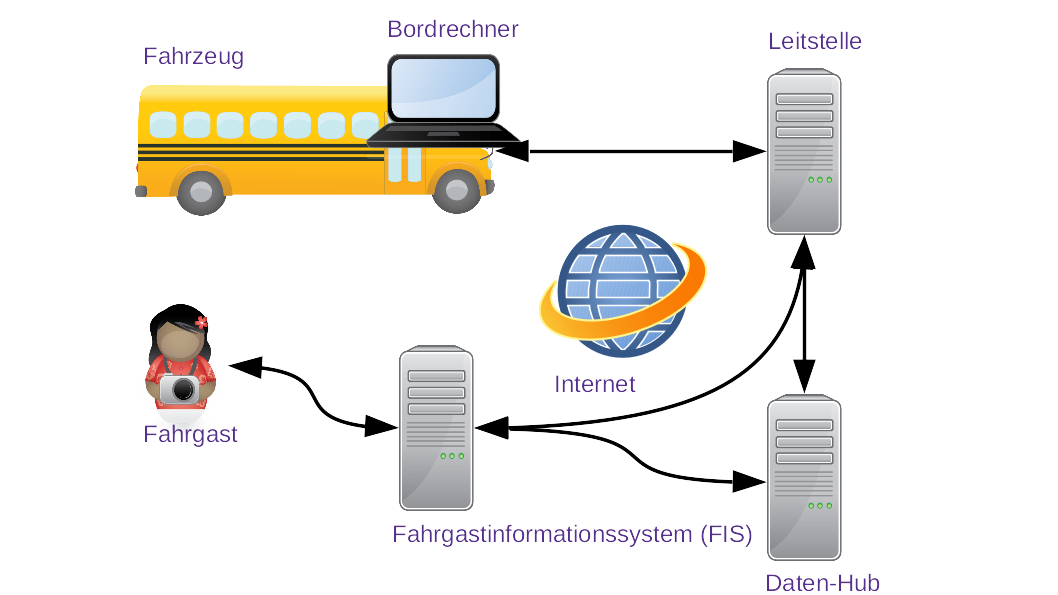
\includegraphics[width=1.1\textwidth]{otm-june-2-2021/public-transport.png}
  \end{center}
\end{frame}


%/*
% * SPDX-FileCopyrightText: 2021 Stefan Begerad <stefan@begerad.de>
% *
% * SPDX-License-Identifier: GPL-3.0-or-later
% */

\begin{frame}{Konventioneller Bordrechner}
  \begin{itemize}
  \item Im Fahrzeug fest verbaut und mit Strom- und Datennetz verbunden
  \item Investitionskosten pro Fahrzeug: etwa 2 bis 3 Tausend Euro
  \item Betriebskosten pro Farhzeug: im Bereich von 1 bis 5 Prozent p.a.
    \begin{itemize}
    \item Lizenskosten
    \item Supportkosten
    \end{itemize}
  \item Interaktion mit
    \begin{itemize}
    \item Fahrzeugnetz bspw. IBIS,
    \item Ticket-Drucker oder -Scanner,
    \item Anzeige für Fahrdienst,
    \item Leitstelle per Analog- oder Digitalfunk (SIM-Karte fuer Mobilfunk)
    \item Ortung per GPS
    \end{itemize}
  \end{itemize}
  
\includegraphics[width=0.5\textwidth]{otm-june-2-2021/bus.png}
\end{frame}



\bgroup

\usebackgroundtemplate{%
\tikz\node[opacity=0.8,inner sep=0] {
   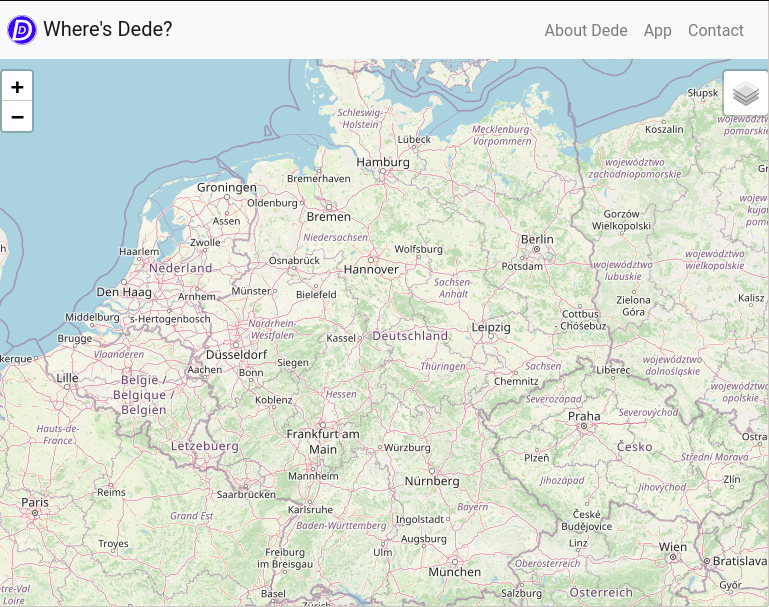
\includegraphics[width=\paperwidth]{dede/dede-map-sh-empty}};
}

%/*
% * SPDX-FileCopyrightText: 2021 Stefan Begerad <stefan@begerad.de>
% *
% * SPDX-License-Identifier: GPL-3.0-or-later
% */

\begin{frame}{Dede Echtzeit-Karte für Deutschland}
\center {\Huge\textbf{Wo sind die Echtzeit-Daten?}}
\center {\huge\textbf{ Wo sind die Fahrzeuge?}}
\end{frame}


\egroup

%/*
% * SPDX-FileCopyrightText: 2021 Stefan Begerad <stefan@begerad.de>
% *
% * SPDX-License-Identifier: GPL-3.0-or-later
% */

\begin{frame}{Herausforderungen bei Echtzeit-Daten in Deutschland}
  \begin{block}{Kosten}
    Hohe Betriebs- und Investitionskosten für IT-Infrastruktur
  \end{block}

  \begin{block}{Organisation}
    Mangel an eigenem IT-Personal bei Verkehrsunternehmen
  \end{block}

  \begin{block}{Standards}
    Einsatz von vielen proprietären Industriestandards
  \end{block}

  \begin{block}{Wettbewerb}
    Fehlender Wettbewerb bei Software- und Systemlieferanten
  \end{block}
\end{frame}



%%/*
% * SPDX-FileCopyrightText: 2021 Stefan Begerad <stefan@begerad.de>
% *
% * SPDX-License-Identifier: GPL-3.0-or-later
% */

\begin{frame}{Verkehrsunternehmen}
  Unternehmen im Personenverkehr in Deutschland:\footnote{VDV Statistik 2019}
  \begin{itemize}
    \item Bus: 272
    \item TRAM\footnote{Personenverkehr mit Straßenbahnen, Stadt- und U-Bahnen oder vergleichbaren Verkehrssystemen}: 76
    \item PVE\footnote{Personenverkehr mit Eisenbahnen}: 113
  \end{itemize}
\end{frame}


%/*
% * SPDX-FileCopyrightText: 2021 Stefan Begerad <stefan@begerad.de>
% *
% * SPDX-License-Identifier: GPL-3.0-or-later
% */

\begin{frame}{Verkehrsmittel}

  \begin{block}{Annahme}
    Ca. 100 Tausend Fahrzeuge im Personenverkehr
  \end{block}

  \begin{columns}

    \begin{column}{0.5\textwidth}
      \minipage[c][0.65\textheight][s]{\columnwidth}
      Verkehrsmittel VDV\footnote{VDV Statistik 2019}:
      \begin{itemize}
      \item Busse: 35633
      \item TRAM: 7257
      \item SPNV\footnote{Schienenpersonennahverkehr}: 15350
      \end{itemize}
      \endminipage
    
    \end{column}

    \begin{column}{0.5\textwidth}
      \minipage[c][0.65\textheight][s]{\columnwidth}
    Verkehrsmittel DESTATIS\footnote{DESTATIS 2013}:
    \begin{itemize}
    \item Busse: 76100, ca. 1/5km2
    \item TRAM: 7500, ca. 1/50km2
    \item SPNV\footnote{Schienenpersonennahverkehr}: 16100, ca. 1/20km2
    \end{itemize}
    \endminipage
    \end{column}

  \end{columns}

\end{frame}



%/*
% * SPDX-FileCopyrightText: 2021 Stefan Begerad <stefan@begerad.de>
% *
% * SPDX-License-Identifier: GPL-3.0-or-later
% */

\begin{frame}{Kosten für Busbordrechner}
  \begin{block}{Weitere Annahmen}
  \begin{itemize}
  \item 2.000 Euro Investitionskosten pro Bus
  \item 5 Prozent gleich 100 Euro Betreiebskosten pro Bus p.a.
  \item 10 Jahre Betriebszeit pro Bus
  \item 5 Jahre Betriebszeit pro Bordrechner
  \end{itemize}
  \end{block}
\end{frame}



%/*
% * SPDX-FileCopyrightText: 2021 Stefan Begerad <stefan@begerad.de>
% *
% * SPDX-License-Identifier: GPL-3.0-or-later
% */

\begin{frame}{Kosten für Bordrechner}
  \begin{itemize}
  \item 100 T Fahrzeuge bei 500 Unternehmen ergeben \textbf{250} Fahrzeuge pro Unternehmen
  \item 2 Bordrechner fodern 6 T Euro Investition pro Fahrzeug
  \item 600 plus 150 Euro Kosten pro Fahrzeug p.a. resultieren aus 10 Jahre Betriebszeit
  \end{itemize}
  \begin{block}{Kosten}
    187,500 Euro pro Verkehrsunternehmen p.a. für Bordrechner
  \end{block}
\end{frame}


%%/*
% * SPDX-FileCopyrightText: 2021 Stefan Begerad <stefan@begerad.de>
% *
% * SPDX-License-Identifier: GPL-3.0-or-later
% */

\begin{frame}{Kosten für Bus mit Dede}
  \begin{itemize}
  \item 1 Smartphone fodert 200 Euro Investition pro Bus
  \item 20 Euro Kosten pro Bus p.a. resultieren aus 10 Jahre Betriebszeit
  \end{itemize}
  \begin{block}{Kosten}
    1.522.000 Euro für Busse mit Dede in Deutschland p.a.
  \end{block}
\end{frame}


\section{Die Dede Echtzeit-Karte}

%/*
% * SPDX-FileCopyrightText: 2021 Stefan Begerad <stefan@begerad.de>
% *
% * SPDX-License-Identifier: GPL-3.0-or-later
% */

\bgroup

\usebackgroundtemplate{%
\tikz\node[opacity=1,inner sep=0] {
   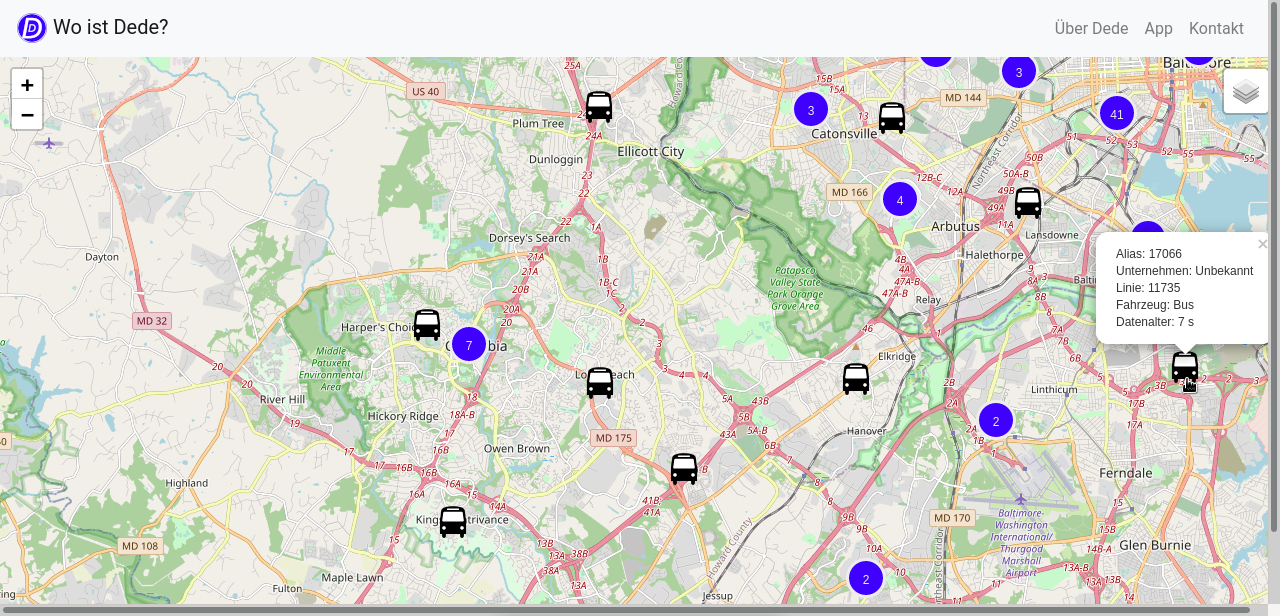
\includegraphics[width=\paperwidth]{dede/dede_real-time_map_crop}};
}

\begin{frame}{Dede Echtzeit-Karte}
\end{frame}

\egroup



\bgroup

\usebackgroundtemplate{%
\tikz\node[opacity=0.1,inner sep=0] {
   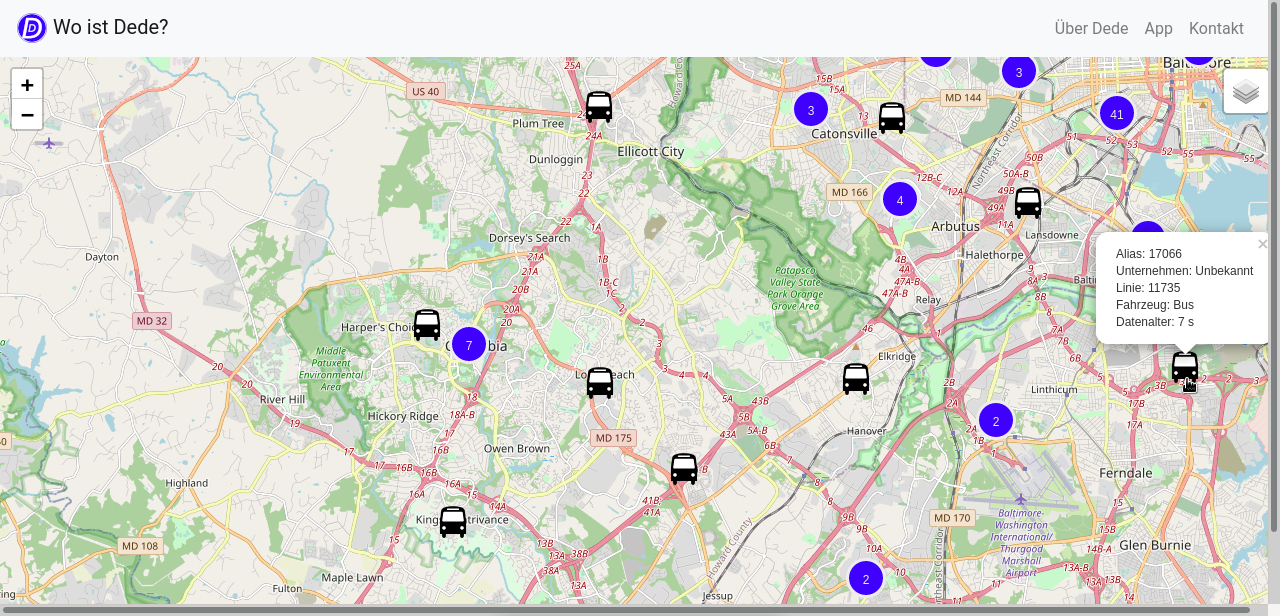
\includegraphics[width=\paperwidth]{dede/dede_real-time_map_crop}};
}

%/*
% * SPDX-FileCopyrightText: 2021 Stefan Begerad <stefan@begerad.de>
% *
% * SPDX-License-Identifier: GPL-3.0-or-later
% */

\begin{frame}{Dede Philosophie}
  Dede: eine freie, unabhängige und universelle Echtzeit-Karte
  \begin{itemize}
  \item FREI: Gemeinschaftsprojejt als freie Software (wie in Redefreiheit und NICHT wie in Freibier;-)) veröffenlicht\footnote{\url{https://github.com/dancesWithCycles/dede-front-end}}
  \item UNABHÄNGIG: weder ausgerüstete Fahrzeugflotte noch eigene IT-Infrastuktur notwendig
  \item UNIVERSELL: beliebige Fahrzeuge wie Bahn, Bus, Car-Sharing, Fahrdienst, Straßenbahn, Tram, Taxi, usw. universell darstellt
  \end{itemize}
\end{frame}


%/*
% * SPDX-FileCopyrightText: 2021 Stefan Begerad <stefan@begerad.de>
% *
% * SPDX-License-Identifier: GPL-3.0-or-later
% */

\begin{frame}{Dede Konzept}
  %alternative alignment to center is left and right
  \begin{center}
    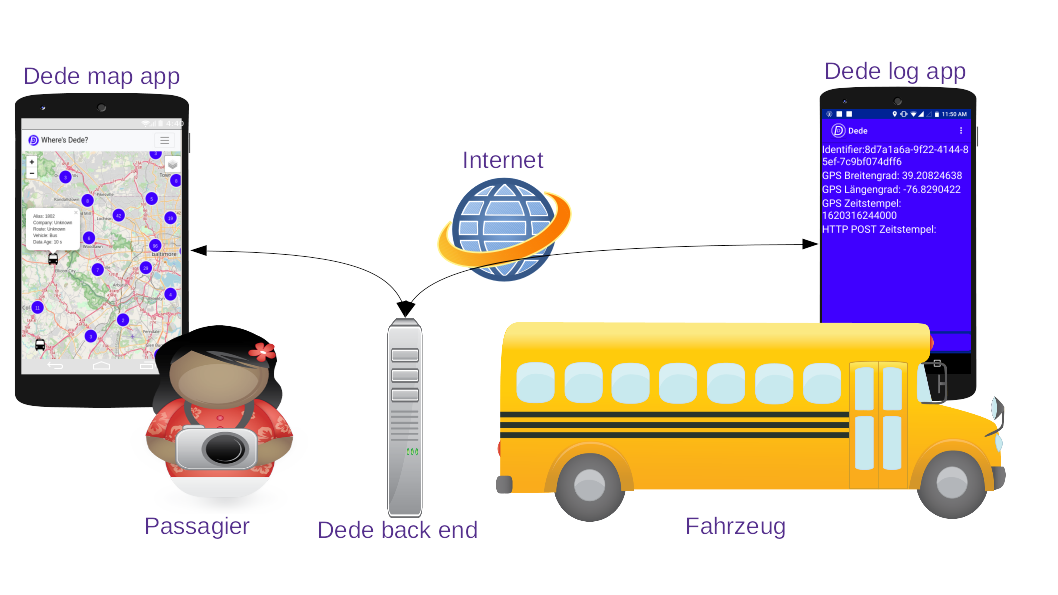
\includegraphics[width=\paperwidth]{dede/dede-concept}
  \end{center}
\end{frame}

\begin{frame}{Dede Konzept}
  Die Dede Echtzeit-Karte besteht aus drei Komponenten:
  \begin{itemize}
  \item Die Dede-App für Smartphones zeichnet die Bewegungsdaten des Fahrzeugs auf und überträgt sie per Internet an den Dede-Server.
  \item Der Dede-Server vermittelt zwischen Dede-App und Dede-Karte, so das die Karte NICHT jede App separat abfragen muss.
  \item Die Dede-Karte visualisiert die Bewegungdaten auf einer Karte in Echtzeit.
  \end{itemize}
\end{frame}


%/*
% * SPDX-FileCopyrightText: 2021 Stefan Begerad <stefan@begerad.de>
% *
% * SPDX-License-Identifier: GPL-3.0-or-later
% */

\begin{frame}{Dede Integration}
  \begin{itemize}
  \item Betrieblich:
    \begin{itemize}
    \item Ein Fahrzeug erscheint in Echtzeit auf der \textbf{Dede Karte}, sobald der Fahrdienst die App \textbf{Dede Bordrechner} aktiviert.
    \item Ein Fahrzeug wird von der \textbf{Dede Karte} in Echtzeit entfernt, sobald der Fahrdienst die App \textbf{Dede Bordrechner} deaktiviert.
      \item In der App \textbf{Dede Bordrechner} kann der Fahrdienst Details zu Betreiber, Nummer und Richtung bei Bedarf eingestellen.
    \end{itemize}
  \item Technisch:
    \begin{itemize}
    \item Pro Fahrzeug ist vom Fahrdienst ein Smartphone mit Android Betriebssystem mitzuführen.
    \item Das Smartphone muss jederzeit aktiv sein mit einer ständigen Stromversorgung und Internet-Verbindung (bspw. per Mobilfunk).
    \end{itemize}
  \end{itemize}
\end{frame}


\egroup

\section*{Danke!}

\begin{frame}{Danke!}
  \center Fragen?
\end{frame}

\end{document}
